\documentclass{ximera}

\begin{document}
	\author{Stitz-Zeager}
	\xmtitle{Exercises for Power Functions}{}

In following exercises, use the given graphs along with Theorem \ref{linearrationalpowergraphs} to graph the given function.  Track at least two points and state the domain and range using interval notation.



\begin{image}[0.75\textwidth]


	\tikz{\begin{axis}[fpplot,xmin=-2,xmax=2,ymax=5]
  		\addplot+[mark=none,domain=-1.2:1.2] (t^3,t^2);
		\node[circle, fill=blue, inner sep=2pt, label=below right:{$( 0,0)$}] at (axis cs: 0,0){};
		\node[circle, fill=blue, inner sep=2pt, label=below right:{$( 1,1)$}] at (axis cs: 1,1){};
		\node[circle, fill=blue, inner sep=2pt, label=below left :{$(-1,1)$}] at (axis cs:-1,1){};

		\node[below left=0.5cm,blue] at (axis cs:0,0) {$f(x)=x^{\frac{2}{3}}$}; 
	\end{axis}
	}
	\hfill
	\tikz{\begin{axis}[fpplot,xmin=-2,xmax=2]
  		\addplot+[mark=none,domain=-0:1.5,xlabel={$t$}] (t,t^pi);
		\node[circle, fill=blue, inner sep=2pt, label=below right:{$( 0,0)$}] at (axis cs: 0,0){};
		\node[circle, fill=blue, inner sep=2pt, label=below right:{$( 1,1)$}] at (axis cs: 1,1){};

		\node[below left=0.5cm,blue] at (axis cs:0,0) {$f(x)=x^{\frac{2}{3}}$}; 
	\end{axis}
	}

\end{image}




\begin{question} $F(x) = (x-2)^{\frac{2}{3}}-1$ \label{powergraphexfirst} 

\begin{solution}

		\tikz{\begin{axis}[fplot,xmin=-2,xmax=6, ymin=-2]
  		\addplot+[mark=none,domain=-1:5] {(abs(x-2))^(2/3) - 1};
		\node[circle, fill=blue, inner sep=2pt, label=below left :{$( 1,0)$}] at (axis cs: 1,0){};
		\node[circle, fill=blue, inner sep=2pt, label=below right:{$( 3,0)$}] at (axis cs: 3,0){};
		\node[circle, fill=blue, inner sep=2pt, label=below      :{$(2,-1)$}] at (axis cs:2,-1){};

		\node[below left=0.5cm,blue,align=left] at (axis cs:0,0) 
		  {$F(x)=(x-2)^{\frac{2}{3}}-1$\\
		  Domain:  $(-\infty, \infty)$, Range:  $[-1, \infty)$}; 
		\end{axis}
		}


\end{solution}
\end{question}



\begin{question} $G(t) = (t+3)^{\pi} +1$ \end{question}




\begin{question} $F(x) = 3-x^{\frac{2}{3}}$  \end{question}
\begin{question} $G(t) = (1-t)^{\pi}-2$  \vphantom{$F(x) = 3-x^{\frac{2}{3}}$ } \end{question}






\begin{question} $F(x) =(2x+5)^{\frac{2}{3}}+1$ \vphantom{$G(t) = \left( \dfrac{t+3}{2}\right)^{\pi}-1$} \end{question}
\begin{question} $G(t) = \left( \dfrac{t+3}{2}\right)^{\pi}-1$ \label{powergraphexlast} \end{question}




In Exercises \ref{findformulaforpowergraphfirst} - \ref{findformulaforpowergraphlast}, find a formula for each function below in the form $F(x) = a(bx-h)^{\frac{2}{3}}+k$.

\smallskip

\textbf{NOTE:}  There may be more than one solution!


\begin{question}  $y=F(x)$ %$F(x) = 2(x-1)^{\frac{2}{3}}-2$
%
	\tikz{\begin{axis}[fpplot,xmin=-2,xmax=4]
  		\addplot+[mark=none,domain=-1.5:1.5] (t^3+1,2*t^2-2);
		\node[circle, fill=blue, inner sep=2pt, label=below left :{$( 0,0)$}] at (axis cs: 0,0){};
		\node[circle, fill=blue, inner sep=2pt, label=below right:{$(1,-2)$}] at (axis cs:1,-2){};
		\node[circle, fill=blue, inner sep=2pt, label=below right:{$( 2,0)$}] at (axis cs: 2,0){};

		% \node[below left=0.5cm,blue] at (axis cs:0,0) {$f(x)=x^{\frac{2}{3}}$}; 
	\end{axis}
	}
 
\end{question}
\begin{question}
$y = F(x)$ %$F(x) =-(x+1)^{\frac{2}{3}} + 4$
%
	\tikz{\begin{axis}[fpplot,xmin=-10,xmax=7,ymax=5]
  		\addplot+[mark=none,domain=-2.1:2.,samples=1000] (t^3-1,4-t^2);
		\node[circle, fill=blue, inner sep=2pt, label=right      :{$( 0,3)$}] at (axis cs: 0,3){};
		\node[circle, fill=blue, inner sep=2pt, label=above left :{$(-1,4)$}] at (axis cs:-1,4){};
		\node[circle, fill=blue, inner sep=2pt, label=below left :{$( 6,0)$}] at (axis cs: 6,0){};
		\node[circle, fill=blue, inner sep=2pt, label=below right:{$(-9,0)$}] at (axis cs:-9,0){};

		% \node[below left=0.5cm,blue] at (axis cs:0,0) {$f(x)=x^{\frac{2}{3}}$}; 
	\end{axis}
	}



\end{question}

For each function in following exercises,

\begin{itemize}

\item Analytically:



\begin{itemize}

\item find the domain.

\item find the axis intercepts.

\item analyze the end behavior.

\end{itemize}



\item Graph the function with help from a graphing utility and determine:



\begin{itemize}

\item  the range.

\item the local extrema, if they exist.

\end{itemize}





\begin{itemize}

\item intervals of increase/decrease.

\item any `unusual steepness' or `local' verticality.

\end{itemize}





\begin{itemize}

\item  vertical asymptotes.

\item  horizontal / slant asymptotes.

\end{itemize}



\item Construct a sign diagram for each function using the intercepts and graph.

\item  Comment on any observed symmetry.


\end{itemize}



\begin{question} $f(x) = x^{\frac{2}{3}}(x - 7)^{\frac{1}{3}}$
\end{question}
\begin{question} $f(x) = x^{\frac{3}{2}}(x - 7)^{\frac{1}{3}}$  
\end{question}
\begin{question} $g(t) = 2t(t+3)^{-\frac{1}{3}}$  
\end{question}
\begin{question} $g(t) = t^{\frac{3}{2}}(t-2)^{-\frac{1}{2}}$  
\end{question}
\begin{question} $f(x) = x^{0.4} (3-x)^{0.6}$  
\end{question}
\begin{question} $f(x) = x^{0.5} (3-x)^{0.5}$  
\end{question}
\begin{question} $g(t) = 4t (9-t^2)^{-\sqrt{2}}$  
\end{question}
\begin{question} $g(t) = 3(t^2+1)^{-\pi}$
\end{question}



% Transformed Exercises with Solutions

\begin{question}
For each function $f(x)$ listed below, compute the average rate of change over the indicated interval.\footnote{See Definition \ref{arc} in Section \ref{AverageRateofChange} for a review of this concept, as needed.}  What trends do you observe?  How do your answers manifest themselves graphically?  Compare the results of this exercise with those of Exercise \ref{monomialarcexercise} in Section \ref{GraphsofPolynomials} and Exercise \ref{laurentarcexercise} in Section \ref{IntroRational}

\[ \begin{array}{|r||c|c|c|c|}  \hline

 f(x) &  [0.9, 1.1] & [0.99, 1.01] &[0.999, 1.001] & [0.9999, 1.0001]  \\ \hline
 x^{\frac{1}{2}} &&&&  \\  \hline
 x^{\frac{2}{3}} &&&&  \\ \hline
 x^{-0.23} &&&&   \\  \hline
 x^{\pi}  &&&&   \\  \hline

\end{array} \]
\begin{solution}
$F(x) = (x-2)^{\frac{2}{3}}-1$ \\

% \begin{tikzpicture}

\begin{axis}[fpplot, xlabel={}, ylabel={}, xmin=-2, xmax=6, ymin=-2, ymax=3, width=160pt, height=100pt]
\node at (axis cs:6,-0.5) {\scriptsize $x$};
\node at (axis cs:0.25,3) {\scriptsize $y$};
\node at (axis cs:3.5,-0.5) {\scriptsize $(3,0)$};
\node at (axis cs:0.5,-0.5) {\scriptsize $(1,0)$};
\node at (axis cs:2,-1.5) {\scriptsize $(2,-1)$};
\addplot[domain=-1.5:1.5] ({t^3+2},{t^2-1});
\addplot[only marks, mark=*, mark size=1.5pt] coordinates {(1,0) (2,-1) (3,0)};
\node at (axis description cs:0.5,-0.12) {Domain:  $(-\infty, \infty)$, Range:  $[-1, \infty)$};
\end{axis}
\end{tikzpicture}
\begin{tikzpicture}

\begin{axis}[fpplot, xlabel={}, ylabel={}, xmin=-2, xmax=6, ymin=-2, ymax=3, width=160pt, height=100pt]
\node at (axis cs:6,-0.5) {\scriptsize $x$};
\node at (axis cs:0.25,3) {\scriptsize $y$};
\node at (axis cs:3.5,-0.5) {\scriptsize $(3,0)$};
\node at (axis cs:0.5,-0.5) {\scriptsize $(1,0)$};
\node at (axis cs:2,-1.5) {\scriptsize $(2,-1)$};
\addplot[domain=-1.5:1.5] ({t^3+2},{t^2-1});
\addplot[only marks, mark=*, mark size=1.5pt] coordinates {(1,0) (2,-1) (3,0)};
\node at (axis description cs:0.5,-0.12) {Domain:  $(-\infty, \infty)$, Range:  $[-1, \infty)$};
\end{axis}
\end{tikzpicture}
\end{solution}

\end{question}

\begin{question}
The \href{http://www.nws.noaa.gov/om/windchill/windchillglossary.shtml}{\underline{National Weather Service}} uses the following formula to calculate the wind chill: \[ W = 35.74 + 0.6215 \, T_{a} - 35.75\, V^{0.16} + 0.4275 \, T_{a} \, V^{0.16}  \] where $W$ is the wind chill temperature in $^{\circ}$F, $T_{a}$ is the air temperature in $^{\circ}$F, and  $V$ is the wind speed in miles per hour.  Note that $W$ is defined only for air temperatures at or lower than $50^{\circ}$F and wind speeds above $3$ miles per hour.

\begin{solution}
$G(t) = (t+3)^{\pi} +1$ \vphantom{$F(x) = (x-2)^{\frac{2}{3}}-1$}\\

% \begin{mfpic}[20]{-7}{1}{0}{5}
\axes
\tlabel[cc](1, -0.5){\scriptsize $t$}
\tlabel[cc](0.5, 5){\scriptsize $y$}
\tlabel[cc](-1,2){\scriptsize $(-2,2)$}
\tlabel[cc](-2.5,0.5){\scriptsize $(-3,1)$}
\penwd{1.25pt}
\arrow  \function{-3,-1.5,0.1}{((x+3)**3.14)+1}
\point[4pt]{(-3,1), (-2,2)}
\tcaption{Domain:  $[-3, \infty)$, Range:  $[1, \infty)$}
\end{mfpic}
\begin{tikzpicture}

\begin{axis}[fplot, xlabel={}, ylabel={}, xmin=-7, xmax=1, ymin=0, ymax=5, width=160pt, height=100pt]
\node at (axis cs:1,-0.5) {\scriptsize $t$};
\node at (axis cs:0.5,5) {\scriptsize $y$};
\node at (axis cs:-1,2) {\scriptsize $(-2,2)$};
\node at (axis cs:-2.5,0.5) {\scriptsize $(-3,1)$};
\addplot[domain=-3:-1.5] {((x+3)^3.14)+1};
\addplot[only marks, mark=*, mark size=1.5pt] coordinates {(-3,1) (-2,2)};
\node at (axis description cs:0.5,-0.12) {Domain:  $[-3, \infty)$, Range:  $[1, \infty)$};
\end{axis}
\end{tikzpicture}



\end{solution}

\end{question}

\begin{question}
Suppose the air temperature is $42^{\circ}$ and the wind speed is $7$ miles per hour. Find the wind chill temperature.  Round your answer to two decimal places.
\begin{solution}
$F(x) = 3-x^{\frac{2}{3}} = (-1)x^{\frac{2}{3}} + 3$  \\

% \begin{mfpic}[20]{-4}{4}{-1}{4}
\axes
\tlabel[cc](4, -0.5){\scriptsize $x$}
\tlabel[cc](0.5, 4){\scriptsize $y$}
\tlabel[cc](1.5,2.25){\scriptsize $(1,2)$}
\tlabel[cc](-1.75,2.25){\scriptsize $(-1,2)$}
\tlabel[cc](0.75,3){\scriptsize $(0,3)$}
\penwd{1.25pt}
\arrow \reverse \arrow \parafcn{-1.5, 1.5,0.1}{(t**3,3-(t**2))}
\point[4pt]{(-1,2), (0,3), (1,2)}
\tcaption{Domain: $(-\infty, \infty)$, Range: $(-\infty,3]$} 
\end{mfpic}
\begin{tikzpicture}

\begin{axis}[fpplot, xlabel={}, ylabel={}, xmin=-4, xmax=4, ymin=-1, ymax=4, width=160pt, height=100pt]
\node at (axis cs:4,-0.5) {\scriptsize $x$};
\node at (axis cs:0.5,4) {\scriptsize $y$};
\node at (axis cs:1.5,2.25) {\scriptsize $(1,2)$};
\node at (axis cs:-1.75,2.25) {\scriptsize $(-1,2)$};
\node at (axis cs:0.75,3) {\scriptsize $(0,3)$};
\addplot[domain=-1.5:1.5] ({t^3},{3-(t^2)});
\addplot[only marks, mark=*, mark size=1.5pt] coordinates {(-1,2) (0,3) (1,2)};
\node at (axis description cs:0.5,-0.12) {Domain: $(-\infty, \infty)$, Range: $(-\infty,3]$};
\end{axis}
\end{tikzpicture}
\end{solution}

\end{question}

\begin{question}
Suppose the air temperature is $37^{\circ}$F and the wind chill temperature is $30^{\circ}$F.  Find the wind speed.  Round your answer to two decimal places.
\begin{solution}
$G(t) = (1-t)^{\pi}-2 = ((-1)t+1)^{\pi}-2$  \vphantom{$F(x) = 3-x^{\frac{2}{3}}$} \\

% \begin{mfpic}[20]{-4}{4}{-3}{2}
\axes
\tlabel[cc](4, -0.5){\scriptsize $t$}
\tlabel[cc](0.5, 2){\scriptsize $y$}
\tlabel[cc](2,-2){\scriptsize $(1,-2)$}
\tlabel[cc](0.75,-1){\scriptsize $(0,-1)$}
\penwd{1.25pt}
\arrow  \reverse \function{-0.5, 1,0.1}{((1-x)**3.14)-2}
\point[4pt]{(0,-1), (1,-2)}
\tcaption{Domain:  $(-\infty, 1]$, Range: $[-2, \infty)$}
\end{mfpic}
\begin{tikzpicture}

\begin{axis}[fplot, xlabel={}, ylabel={}, xmin=-4, xmax=4, ymin=-3, ymax=2, width=160pt, height=100pt]
\node at (axis cs:4,-0.5) {\scriptsize $t$};
\node at (axis cs:0.5,2) {\scriptsize $y$};
\node at (axis cs:2,-2) {\scriptsize $(1,-2)$};
\node at (axis cs:0.75,-1) {\scriptsize $(0,-1)$};
\addplot[domain=-0.5:1] {((1 - x)^3.14) - 2};
\addplot[only marks, mark=*, mark size=1.5pt] coordinates {(0,-1) (1,-2)};
\node at (axis description cs:0.5,-0.12) {Domain:  $(-\infty, 1]$, Range: $[-2, \infty)$};
\end{axis}
\end{tikzpicture}


\end{solution}

\end{question}

\begin{question}
Use the formula from Exercise \ref{WindChillTemperature} to find an expression for the wind chill temperature as a function of the wind speed, $W(V)$.
\begin{solution}
$F(x) =(2x+5)^{\frac{2}{3}}+1$ \vphantom{$G(t) = \left( \dfrac{t+3}{2}\right)^{\pi}-1$}  \\

% \begin{mfpic}[20]{-6.5}{1.5}{-1}{4}
\axes
\tlabel[cc](1.5, -0.5){\scriptsize $x$}
\tlabel[cc](0.5, 4){\scriptsize $y$}
\tlabel[cc](-4,1.75){\scriptsize $(-3,2)$}
\tlabel[cc](-2.5,0.5){\scriptsize $\left(-\frac{5}{2},1 \right)$}
\tlabel[cc](-1,1.75){\scriptsize $(-2,2)$}
\penwd{1.25pt}
\arrow \reverse \arrow \parafcn{-1.6, 1.6,0.1}{( 0.5*( (t**3)-5),(t**2)+1)}
\point[4pt]{(-3,2), (-2.5,1), (-2,2)}
\tcaption{Domain: $(-\infty, \infty)$, Range: $[1, \infty)$}
\end{mfpic}
\begin{tikzpicture}

\begin{axis}[fpplot, xlabel={}, ylabel={}, xmin=-6.5, xmax=1.5, ymin=-1, ymax=4, width=160pt, height=100pt]
\node at (axis cs:1.5,-0.5) {\scriptsize $x$};
\node at (axis cs:0.5,4) {\scriptsize $y$};
\node at (axis cs:-4,1.75) {\scriptsize $(-3,2)$};
\node at (axis cs:-2.5,0.5) {\scriptsize $\left(-\frac{5}{2},1 \right)$};
\node at (axis cs:-1,1.75) {\scriptsize $(-2,2)$};
\addplot[domain=-1.6:1.6] ({0.5*((t^3)-5)},{(t^2)+1});
\addplot[only marks, mark=*, mark size=1.5pt] coordinates {(-3,2) (-2.5,1) (-2,2)};
\node at (axis description cs:0.5,-0.12) {Domain: $(-\infty, \infty)$, Range: $[1, \infty)$};
\end{axis}
\end{tikzpicture}
\end{solution}

\end{question}

\begin{question}
Solve $W(V) = 0$, round your answer to two decimal places,  and interpret.
\begin{solution}
$G(t) = \left( \dfrac{t+3}{2}\right)^{\pi}-1= \left( \frac{1}{2} \, t + \frac{3}{2}\right)^{\pi} -1$\\

% \begin{tikzpicture}

\begin{axis}[fplot, xlabel={}, ylabel={}, xmin=-4, xmax=4, ymin=-2, ymax=3, width=160pt, height=100pt]
\node at (axis cs:4,-0.5) {\scriptsize $t$};
\node at (axis cs:0.5,3) {\scriptsize $y$};
\node at (axis cs:-3,-1.5) {\scriptsize $(-3,-1)$};
\node at (axis cs:-1.5,0.5) {\scriptsize $(-1,0)$};
\addplot[domain=-3:-0.2] {(( (x+3)/2 )^3.14) - 1};
\addplot[only marks, mark=*, mark size=1.5pt] coordinates {(-3,-1) (-1,0)};
\node at (axis description cs:0.5,-0.12) {Domain:  $[-3, \infty)$, Range: $[-1, \infty)$};
\end{axis}
\end{tikzpicture}
\begin{tikzpicture}

\begin{axis}[fplot, xlabel={}, ylabel={}, xmin=-4, xmax=4, ymin=-2, ymax=3, width=160pt, height=100pt]
\node at (axis cs:4,-0.5) {\scriptsize $t$};
\node at (axis cs:0.5,3) {\scriptsize $y$};
\node at (axis cs:-3,-1.5) {\scriptsize $(-3,-1)$};
\node at (axis cs:-1.5,0.5) {\scriptsize $(-1,0)$};
\addplot[domain=-3:-0.2] {(( (x+3)/2 )^3.14) - 1};
\addplot[only marks, mark=*, mark size=1.5pt] coordinates {(-3,-1) (-1,0)};
\node at (axis description cs:0.5,-0.12) {Domain:  $[-3, \infty)$, Range: $[-1, \infty)$};
\end{axis}
\end{tikzpicture}


\end{solution}

\end{question}

\begin{question}
Graph the function $W$ using a graphing utility and check your answer to part \ref{WindChill0}.
\begin{solution}
One solution is: $F(x) = 2(x-1)^{\frac{2}{3}}-2$
\end{solution}

\end{question}

\begin{question}
Determine the path that Fritzy will take if he runs exactly twice as fast as Chewbacca;  that is, $v_{\mbox{\tiny$2$}} = 2v_{\mbox{\tiny$1$}}$. Use your calculator to graph this path for $x \geq 0$.  What is the significance of the $y$-intercept of the graph?
\begin{solution}
One solution is: $F(x) =-(x+1)^{\frac{2}{3}} + 4$


\end{solution}

\end{question}

\begin{question}
Determine the path Fritzy will take if Chewbacca runs exactly twice as fast as he does;  that is, $v_{\mbox{\tiny$1$}} = 2v_{\mbox{\tiny$2$}}$.  Use a graphing utility to graph this path for $x > 0$.  Describe the behavior of $y$ as $x \rightarrow 0^{+}$ and interpret this physically.
\begin{solution}
$f(x) = x^{\frac{2}{3}}(x - 7)^{\frac{1}{3}}$\\
Domain: $(-\infty, \infty)$\\
Intercepts: $(0,0)$, $(7,0)$\\
Graph: \\

% \begin{mfpic}[10]{-4}{10}{-5}{5.5}
\axes
\tlabel[cc](10,-0.5){\scriptsize $x$}
\tlabel[cc](0.5,5.5){\scriptsize $y$}
\tlabel[cc](5,-5){\scriptsize $\approx (4.667, -3.704)$}
\xmarks{-3 step 1 until 9}
\ymarks{-4 step 1 until 5}
\tlpointsep{4pt}
\tiny
\axislabels {x}{{$-3 \hspace{6pt}$} -3, {$-2 \hspace{6pt}$} -2, {$-1 \hspace{6pt}$} -1, {$1$} 1, {$2$} 2, {$3$} 3, {$4$} 4, {$5$} 5, {$6$} 6,  {$8$} 8, {$9$} 9}
\axislabels {y}{{$-4$} -4, {$-3$} -3, {$-2$} -2,  {$1$} 1, {$2$} 2, {$3$} 3, {$4$} 4, {$5$} 5}
\normalsize
\point[4pt]{(0,0), (7,0), (4.667, -3.704)}
\dashed \polyline{(-3, -5.33), (9, 6.67)}
\penwd{1.25pt}
\arrow \reverse \function{-3,0,0.1}{-((x**2)**(1/3))*((7 - x)**(1/3))}
\function{0,7,0.1}{-((x**2)**(1/3))*((7 - x)**(1/3))}
\arrow \function{7,9,0.1}{((x**2)**(1/3))*((x - 7)**(1/3))}
\end{mfpic}
\begin{tikzpicture}

\begin{axis}[fplot, xlabel={}, ylabel={}, xmin=-4, xmax=10, ymin=-5, ymax=5.5, width=140pt, height=105pt,
  xtick={-3,-2,-1,1,2,3,4,5,6,8,9},
  xticklabels={$-3 \hspace{6pt}$,$-2 \hspace{6pt}$,$-1 \hspace{6pt}$,{$1$},{$2$},{$3$},{$4$},{$5$},{$6$},{$8$},{$9$}},
  ytick={-4,-3,-2,1,2,3,4,5},
  yticklabels={$-4$,$-3$,$-2$,{$1$},{$2$},{$3$},{$4$},{$5$}}
]
\node at (axis cs:10,-0.5) {\scriptsize $x$};
\node at (axis cs:0.5,5.5) {\scriptsize $y$};
\node at (axis cs:5,-5) {\scriptsize $\approx (4.667, -3.704)$};
\addplot[dashed] coordinates {(-3,-5.33) (9,6.67)};
\addplot[only marks, mark=*, mark size=1.5pt] coordinates {(0,0) (7,0) (4.667,-3.704)};
\addplot[domain=-3:0] {-((x^2)^(1/3))*((7 - x)^(1/3))};
\addplot[domain=0:7] {-((x^2)^(1/3))*((7 - x)^(1/3))};
\addplot[domain=7:9] {((x^2)^(1/3))*((x - 7)^(1/3))};
\end{axis}
\end{tikzpicture}


\vfill


$\ds{\lim_{x \rightarrow - \infty} f(x) = - \infty}$, $\ds{\lim_{x \rightarrow \infty} f(x) = \infty}$\footnote{Using Calculus it can be shown that $y = x - \frac{7}{3}$ is a slant asymptote of this graph.}\\
Range: $(-\infty, \infty)$\\
Local minimum: $\approx (4.667, -3.704)$\\
Local maximum: $(0,0)$ (this is a cusp) \\
Increasing: $(-\infty, 0]$, $\approx [4.667, \infty)$\\
Decreasing: $[0, 4.667]$\\
Unusual steepness at $x = 7$\\

Sign Diagram:\\

\smallskip

% 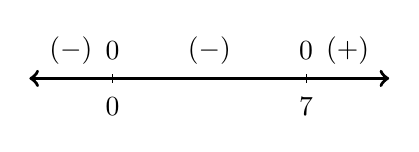
\begin{tikzpicture}[x=10pt,y=10pt]
\draw[<->, line width=1.25pt] (-3,0) -- (10,0);
\foreach \xx in {0,7} {\draw (\xx,-0.15) -- (\xx,0.15);}
\node at (-1.5,1){$(-)$};
\node at (0,-1){$0$};
\node at (0,1){$0$};
\node at (3.5,1){$(-)$};
\node at (7,-1){$7$};
\node at (7,1){$0$};
\node at (8.5,1){$(+)$};
\end{tikzpicture}
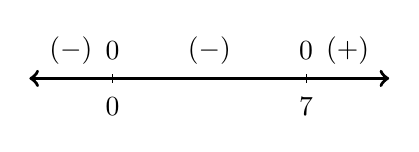
\begin{tikzpicture}[x=10pt,y=10pt]
\draw[<->, line width=1.25pt] (-3,0) -- (10,0);
\foreach \xx in {0,7} {\draw (\xx,-0.15) -- (\xx,0.15);}
\node at (-1.5,1){$(-)$};
\node at (0,-1){$0$};
\node at (0,1){$0$};
\node at (3.5,1){$(-)$};
\node at (7,-1){$7$};
\node at (7,1){$0$};
\node at (8.5,1){$(+)$};
\end{tikzpicture}
\end{solution}

\end{question}

\begin{question}
With the help of your classmates, generalize parts (a) and (b) to two cases:  $v_{\mbox{\tiny$2$}} > v_{\mbox{\tiny$1$}}$ and $v_{\mbox{\tiny$2$}} < v_{\mbox{\tiny$1$}}$.   We will discuss the case of $v_{\mbox{\tiny$1$}} = v_{\mbox{\tiny$2$}}$ in Exercise \ref{pursuitlog} in Section \ref{ExpLogApplications}.
\begin{solution}
$f(x) = x^{\frac{3}{2}}(x - 7)^{\frac{1}{3}}$\\
Graph: \\
% \begin{tikzpicture}

\begin{axis}[fplot, xlabel={}, ylabel={}, xmin=-1, xmax=8.5, ymin=-20, ymax=30, width=142.5pt, height=150pt,
  xtick={2,3,4,5,6,8},
  xticklabels={{$2$},{$3$},{$4$},{$5$},{$6$},{$8$}},
  ytick={-15,-10,-5,5,10,15,20,25},
  yticklabels={{$-15$},{$-10$},{$-5$},{$5$},{$10$},{$15$},{$20$},{$25$}}
]
\node at (axis cs:8.5,-3) {\scriptsize $x$};
\node at (axis cs:0.5,30) {\scriptsize $y$};
\node at (axis cs:6,-18) {\scriptsize $\approx (5.727, -14.854)$};
\addplot[only marks, mark=*, mark size=1.5pt] coordinates {(0,0) (7,0) (5.727,-14.854)};
\addplot[domain=0:7] {-(x^1.5)*((7 - x)^(1/3))};
\addplot[domain=7:8.5] {(x^1.5)*((x - 7)^(1/3))};
\end{axis}
\end{tikzpicture}
\begin{tikzpicture}

\begin{axis}[fplot, xlabel={}, ylabel={}, xmin=-1, xmax=8.5, ymin=-20, ymax=30, width=142.5pt, height=150pt,
  xtick={2,3,4,5,6,8},
  xticklabels={{$2$},{$3$},{$4$},{$5$},{$6$},{$8$}},
  ytick={-15,-10,-5,5,10,15,20,25},
  yticklabels={{$-15$},{$-10$},{$-5$},{$5$},{$10$},{$15$},{$20$},{$25$}}
]
\node at (axis cs:8.5,-3) {\scriptsize $x$};
\node at (axis cs:0.5,30) {\scriptsize $y$};
\node at (axis cs:6,-18) {\scriptsize $\approx (5.727, -14.854)$};
\addplot[only marks, mark=*, mark size=1.5pt] coordinates {(0,0) (7,0) (5.727,-14.854)};
\addplot[domain=0:7] {-(x^1.5)*((7 - x)^(1/3))};
\addplot[domain=7:8.5] {(x^1.5)*((x - 7)^(1/3))};
\end{axis}
\end{tikzpicture}



\vfill


Domain: $[0, \infty)$\\
Intercepts: $(0,0)$, $(7,0)$\\
$\ds{\lim_{x \rightarrow \infty} f(x) = \infty}$\\
Range:  $\approx [-14.854, \infty)$\\
Local minimum:  $\approx (5.727, -14.854)$\\
Increasing: $\approx [5.727, \infty)$\\
Decreasing: $\approx [0, 5.727]$\\
Unusual steepness at $x = 7$\\
Sign Diagram:\\

\smallskip

% 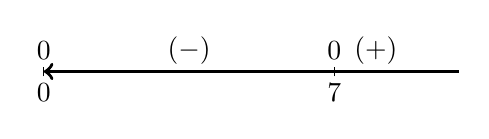
\begin{tikzpicture}[x=15pt,y=15pt]
\draw[<-, line width=1.25pt] (0,0) -- (10,0);
\foreach \xx in {0,7} {\draw (\xx,-0.12) -- (\xx,0.12);}
\node at (0,-0.5){$0$};
\node at (0,0.5){$0$};
\node at (3.5,0.5){$(-)$};
\node at (7,-0.5){$7$};
\node at (7,0.5){$0$};
\node at (8,0.5){$(+)$};
\end{tikzpicture}
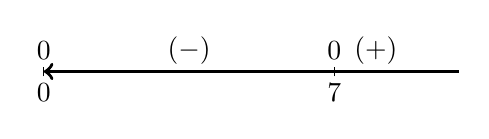
\begin{tikzpicture}[x=15pt,y=15pt]
\draw[<-, line width=1.25pt] (0,0) -- (10,0);
\foreach \xx in {0,7} {\draw (\xx,-0.12) -- (\xx,0.12);}
\node at (0,-0.5){$0$};
\node at (0,0.5){$0$};
\node at (3.5,0.5){$(-)$};
\node at (7,-0.5){$7$};
\node at (7,0.5){$0$};
\node at (8,0.5){$(+)$};
\end{tikzpicture}





\end{solution}

\end{question}

\end{document}